\documentclass{standalone}
\usepackage{tikz}
\begin{document}
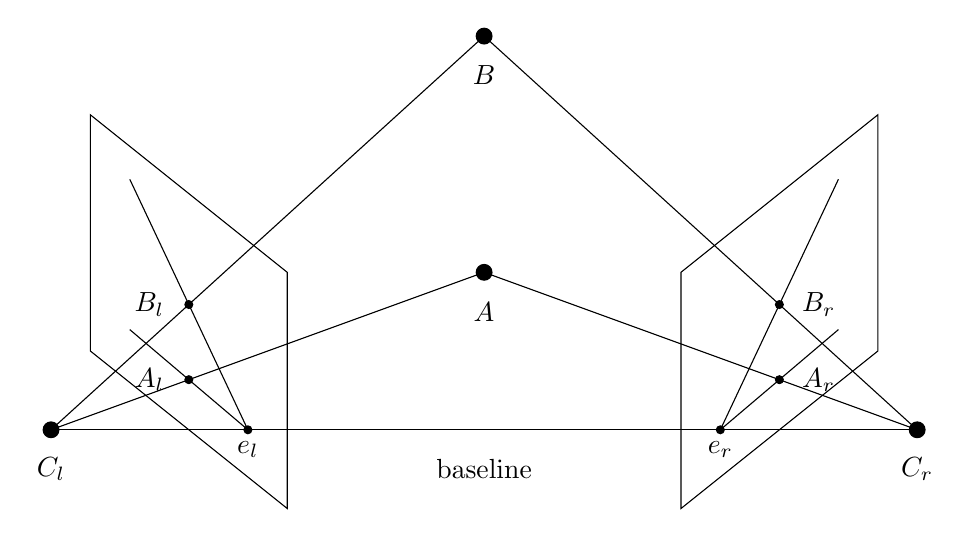
\begin{tikzpicture}[scale=0.5]
	% cameras
	\draw[fill] (-11,-1) circle [radius=0.2];
	\draw[fill] ( 11,-1) circle [radius=0.2];
	\draw (-11,-1) -- (11, -1);
	\node at (0, -2) { baseline };

	\node at (-11,-2) {$C_l$};
	\node at ( 11,-2) {$C_r$};

	% planes
	\draw (-10,1) -- (-10,7) -- (-5,3) -- (-5,-3) -- cycle;
	\draw ( 10,1) -- ( 10,7) -- ( 5,3) -- ( 5,-3) -- cycle;

	% 3d pts
	\draw[fill] ( 0,3) circle [radius=0.2];
	\draw[fill] ( 0,9) circle [radius=0.2];
	\node at (0,2) {$A$};
	\node at (0,8) {$B$};

	% origins via pts
	\draw (-11,-1) -- (0,3) -- (11,-1);
	\draw (-11,-1) -- (0,9) -- (11,-1);

	% epis
	\draw[fill] (-6,-1) circle [radius=0.1];
	\draw[fill] (6,-1) circle [radius=0.1];
	\node at (-6,-1.5) { $e_l$ };
	\node at (6,-1.5) { $e_r$ };

	% projections
	\draw[fill] (-7.5,0.2727) circle [radius=0.1];
	\draw[fill] (-7.5,2.1818) circle [radius=0.1];
	\node at (-8.5, 0.2727) {$A_l$};
	\node at (-8.5, 2.1818) {$B_l$};
	% lines from epis
	\draw (-6,-1) -- +(-2*1.5,2*1.2727);%(-7.5,0.2727);
	\draw (-6,-1) -- +(-2*1.5,2*3.1818);%(-7.5,2.1818);

	\draw[fill] (7.5,0.2727) circle [radius=0.1];
	\draw[fill] (7.5,2.1818) circle [radius=0.1];
	\node at (8.5, 0.2727) {$A_r$};
	\node at (8.5, 2.1818) {$B_r$};
	\draw (6,-1) -- +(2*1.5,2*1.2727);%(7.5,0.2727);
	\draw (6,-1) -- +(2*1.5,2*3.1818);%(7.5,2.1818);
\end{tikzpicture}
\end{document}
